\documentclass[12pt,a4paper]{article}
\usepackage{amsmath,amsfonts}
\usepackage[utf8]{inputenc}
\usepackage[T1]{fontenc}
\usepackage{hyperref}
\usepackage{graphicx}
\usepackage[top=3cm,bottom=3cm,left=3cm,right=3cm]{geometry}

\title{Result of crossover and mutation operations on fitness values}
\author{Witold Bołt <\href{mailto:witold.bolt@hope.art.pl}{witold.bolt@hope.art.pl}>}
\date{\today}

\begin{document}
\maketitle

\section{What do we measure?}
We measure the effect of different genetic operations on resulting fitness values, to check if iterative application of those operations can result in fitness growth.

In case of cross-over we take a pair of individuals (rules). We measure the fitness of both individuals than apply crossover and calculate fitness values once again. We then compare the initial sum of fitness values with the resulting sum.

Despite the fact that mutations are applied independently to each individual, we also calculate our statistics on the same pair as in case of cross-over to enable cumulative analysis (crossover + mutation). So in case of mutations we also calculate a sum of fitness values before and after mutations for the same pairs of individuals as in cross-over case.

\section{Experimental results}

\subsection{Experiment 1}
Here are the experiment parameters:

\begin{verbatim}
Rule to be found: 2294967295 at radius: 2
Radius range: [1, 3]
Upscale probability: 0.05
Downscale probability: 0.05
Population count: 500
Mutation probability: 0.2
Max iteration count: 500
Space size: 79
Time frames: 80
Keep elite: true
Elite size: 4 individuals
\end{verbatim}

The overall results of this evolution is shown on picture \ref{pic-e1-results}. The measured effect of cross-over, mutation, and cross-over + mutation is shown on pictures: \ref{pic-e1-cs}, \ref{pic-e1-ms}, \ref{pic-e1-cms}.


\begin{figure}
\centering
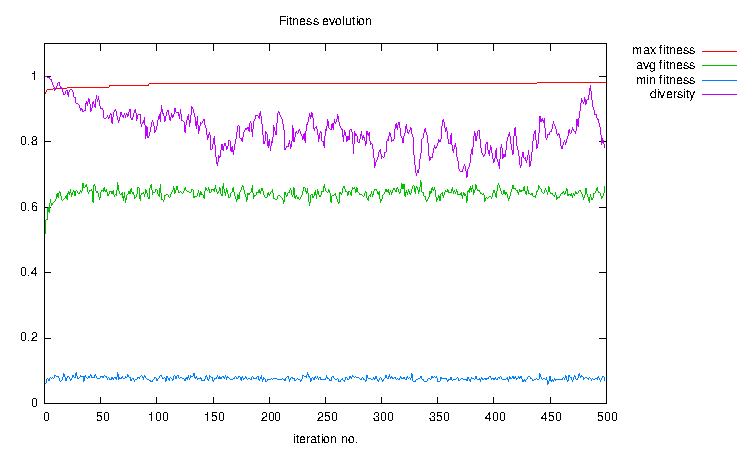
\includegraphics[width=0.8\textwidth]{results/1/1.pdf}
\caption{Experiment 1: Evolution results}
\label{pic-e1-results}
\end{figure}

\begin{figure}
\centering
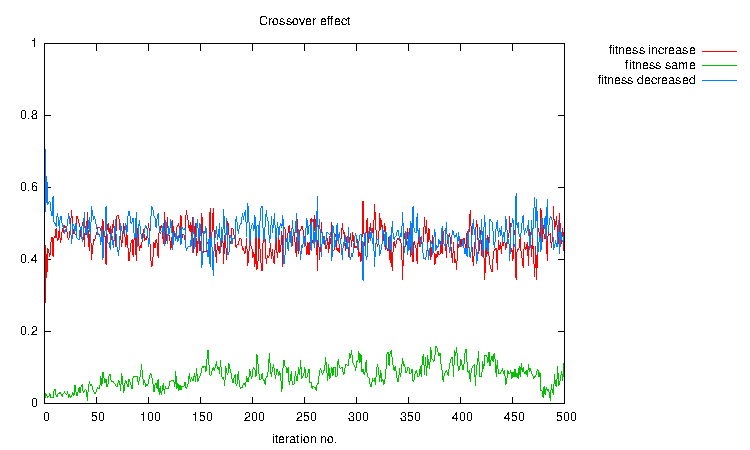
\includegraphics[width=0.8\textwidth]{results/1/1-cs.pdf}
\caption{Experiment 1: Crossover effect}
\label{pic-e1-cs}
\end{figure}

\begin{figure}
\centering
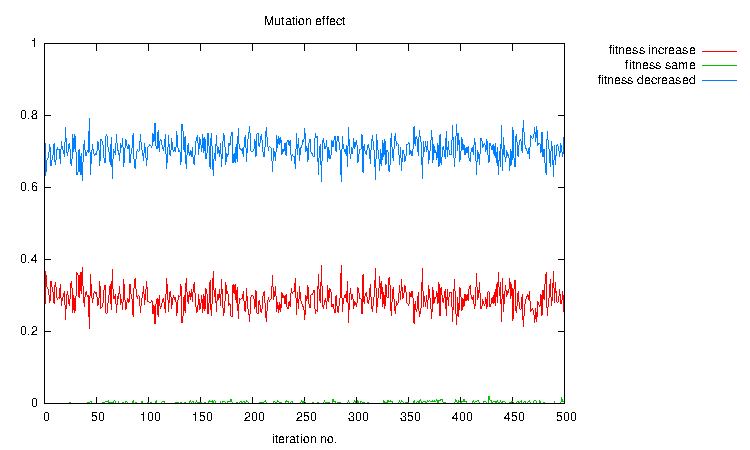
\includegraphics[width=0.8\textwidth]{results/1/1-ms.pdf}
\caption{Experiment 1: Mutation effect}
\label{pic-e1-ms}
\end{figure}

\begin{figure}
\centering
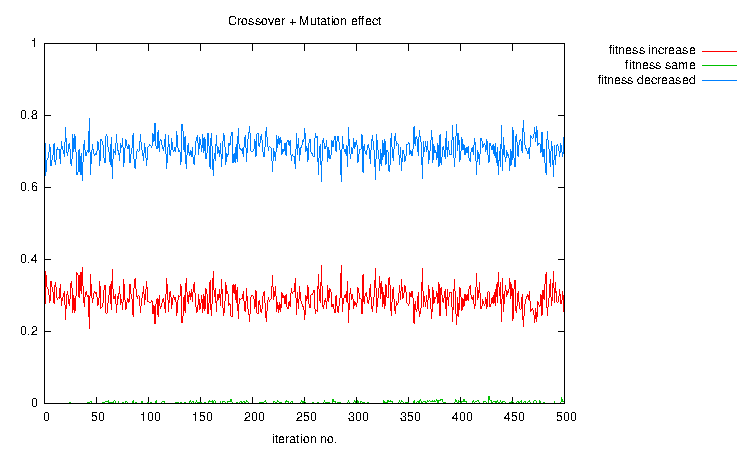
\includegraphics[width=0.8\textwidth]{results/1/1-cms.pdf}
\caption{Experiment 1: Total effect}
\label{pic-e1-cms}
\end{figure}

\subsection{Experiment 2}
Experiment 2 is a copy of experiment 1, but without elite forced survival.

\begin{verbatim}
Rule to be found: 2294967295 at radius: 2
Radius range: [1, 3]
Upscale probability: 0.05
Downscale probability: 0.05
Population count: 500
Mutation probability: 0.2
Max iteration count: 500
Space size: 79
Time frames: 80
Keep elite: false
Elite size: 0 individuals
\end{verbatim}

The overall results of this evolution is shown on picture \ref{pic-e2-results}. The measured effect of cross-over, mutation, and cross-over + mutation is shown on pictures: \ref{pic-e2-cs}, \ref{pic-e2-ms}, \ref{pic-e2-cms}.

\begin{figure}
\centering
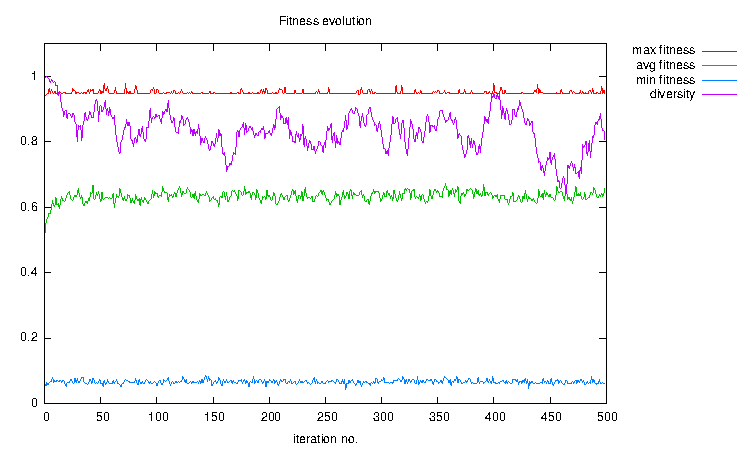
\includegraphics[width=0.8\textwidth]{results/2/1.pdf}
\caption{Experiment 2: Evolution results}
\label{pic-e2-results}
\end{figure}

\begin{figure}
\centering
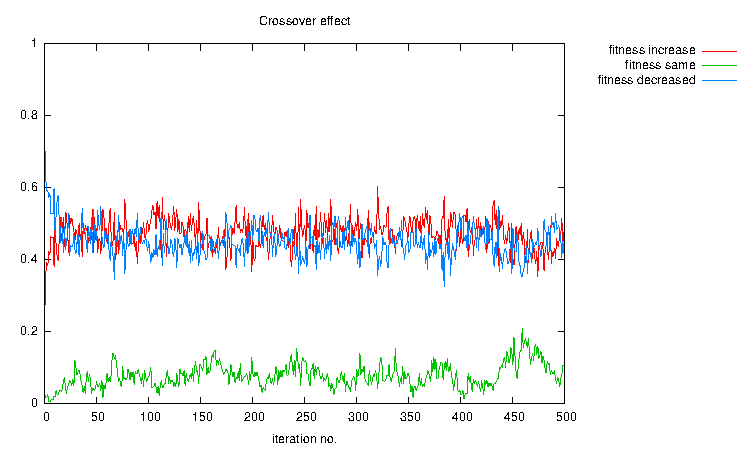
\includegraphics[width=0.8\textwidth]{results/2/1-cs.pdf}
\caption{Experiment 2: Crossover effect}
\label{pic-e2-cs}
\end{figure}

\begin{figure}
\centering
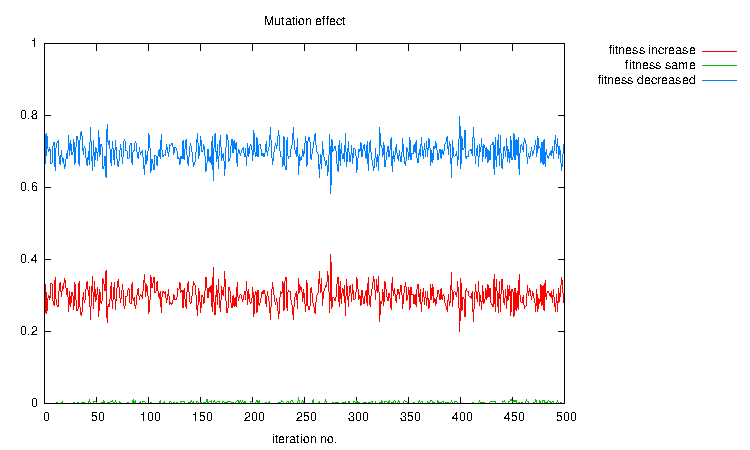
\includegraphics[width=0.8\textwidth]{results/2/1-ms.pdf}
\caption{Experiment 2: Mutation effect}
\label{pic-e2-ms}
\end{figure}

\begin{figure}
\centering
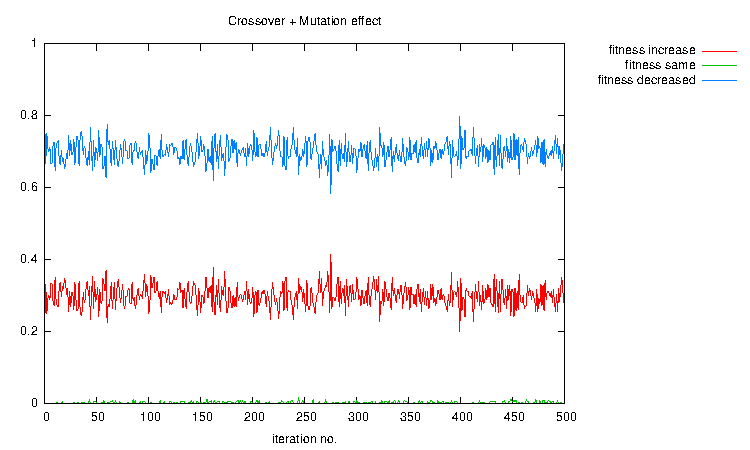
\includegraphics[width=0.8\textwidth]{results/2/1-cms.pdf}
\caption{Experiment 2: Total effect}
\label{pic-e2-cms}
\end{figure}



\subsection{Experiment 3}
Experiment 3 is a copy of experiment 1, but with mutation probabilities increased.

\begin{verbatim}
Rule to be found: 2294967295 at radius: 2
Radius range: [1, 3]
Upscale probability: 0.2
Downscale probability: 0.2
Population count: 500
Mutation probability: 0.3
Max iteration count: 500
Space size: 79
Time frames: 80
Keep elite: true
Elite size: 4 individuals
\end{verbatim}

The overall results of this evolution is shown on picture \ref{pic-e3-results}. The measured effect of cross-over, mutation, and cross-over + mutation is shown on pictures: \ref{pic-e3-cs}, \ref{pic-e3-ms}, \ref{pic-e3-cms}.

\begin{figure}
\centering
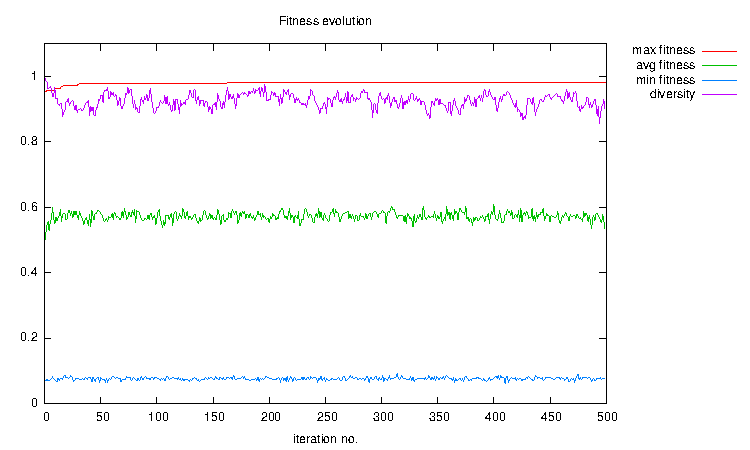
\includegraphics[width=0.8\textwidth]{results/3/1.pdf}
\caption{Experiment 3: Evolution results}
\label{pic-e3-results}
\end{figure}

\begin{figure}
\centering
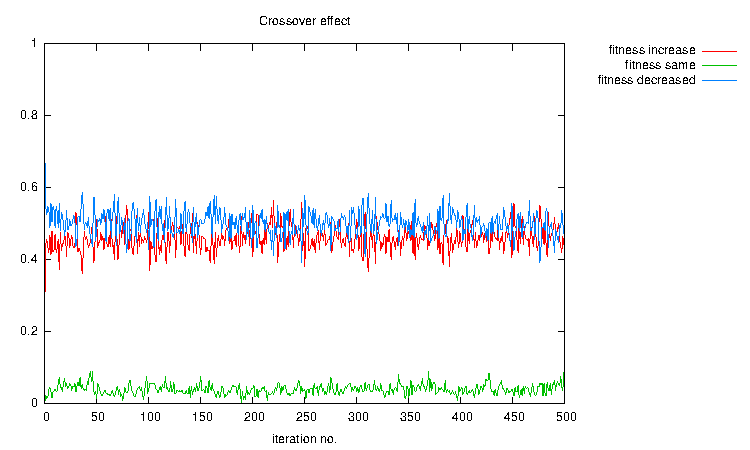
\includegraphics[width=0.8\textwidth]{results/3/1-cs.pdf}
\caption{Experiment 3: Crossover effect}
\label{pic-e3-cs}
\end{figure}

\begin{figure}
\centering
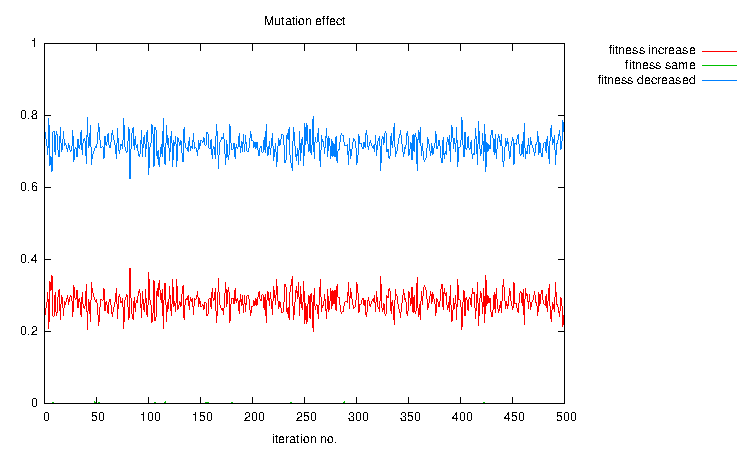
\includegraphics[width=0.8\textwidth]{results/3/1-ms.pdf}
\caption{Experiment 3: Mutation effect}
\label{pic-e3-ms}
\end{figure}

\begin{figure}
\centering
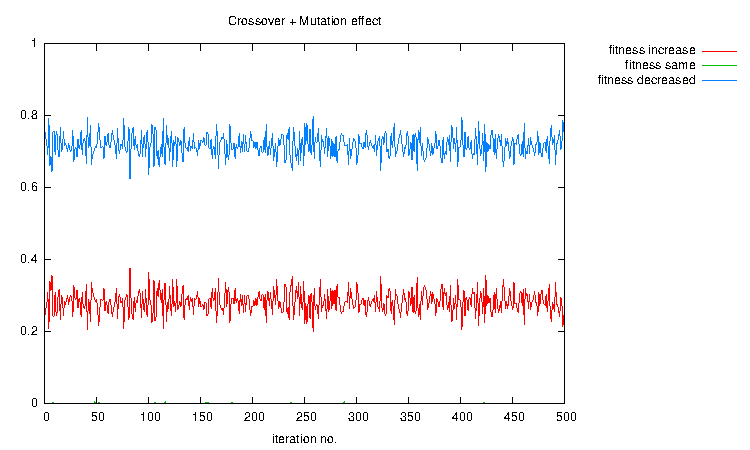
\includegraphics[width=0.8\textwidth]{results/3/1-cms.pdf}
\caption{Experiment 3: Total effect}
\label{pic-e3-cms}
\end{figure}




\subsection{Experiment 4}
Experiment 4 is a copy of experiment 2, but with mutation probabilities increased.

\begin{verbatim}
Rule to be found: 2294967295 at radius: 2
Radius range: [1, 3]
Upscale probability: 0.2
Downscale probability: 0.2
Population count: 500
Mutation probability: 0.3
Max iteration count: 500
Space size: 79
Time frames: 80
Keep elite: false
Elite size: 0 individuals
\end{verbatim}

The overall results of this evolution is shown on picture \ref{pic-e4-results}. The measured effect of cross-over, mutation, and cross-over + mutation is shown on pictures: \ref{pic-e4-cs}, \ref{pic-e4-ms}, \ref{pic-e4-cms}.

\begin{figure}
\centering
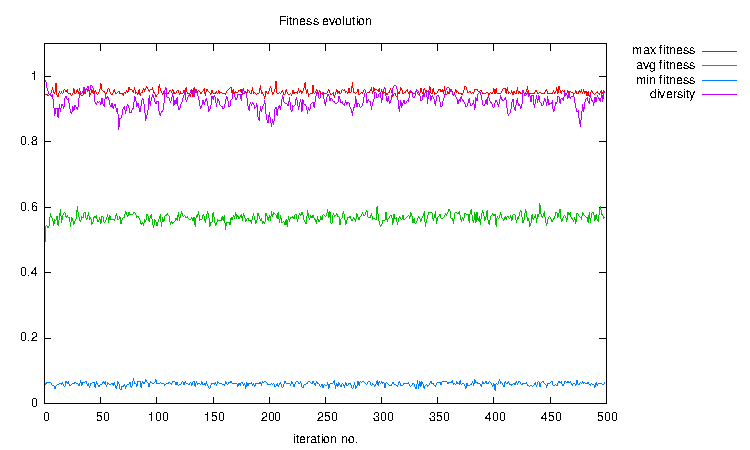
\includegraphics[width=0.8\textwidth]{results/4/1.pdf}
\caption{Experiment 4: Evolution results}
\label{pic-e4-results}
\end{figure}

\begin{figure}
\centering
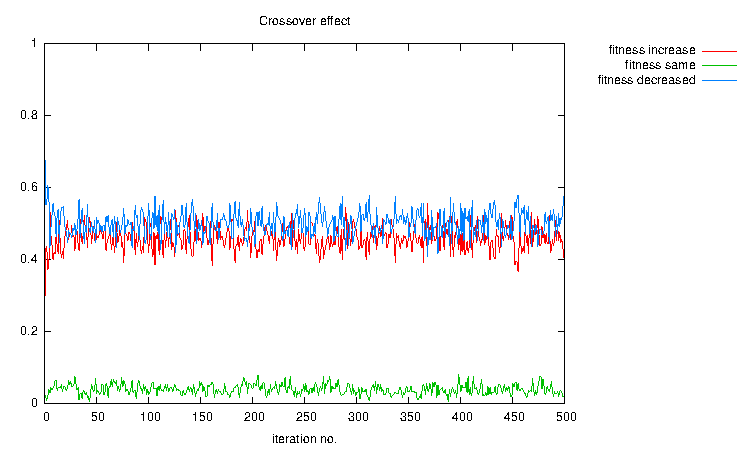
\includegraphics[width=0.8\textwidth]{results/4/1-cs.pdf}
\caption{Experiment 4: Crossover effect}
\label{pic-e4-cs}
\end{figure}

\begin{figure}
\centering
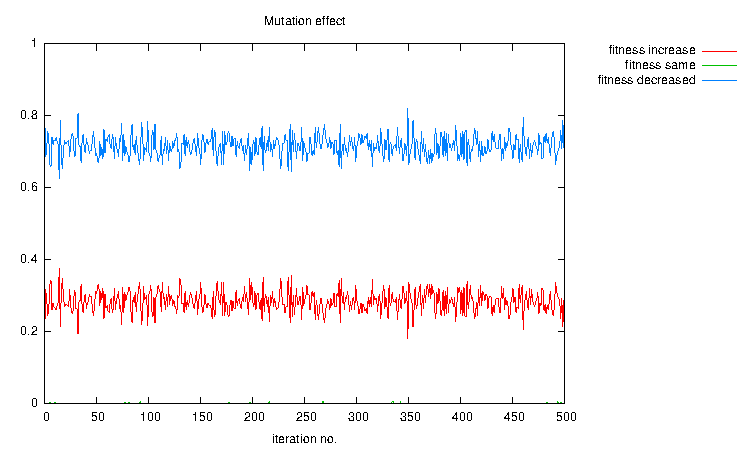
\includegraphics[width=0.8\textwidth]{results/4/1-ms.pdf}
\caption{Experiment 4: Mutation effect}
\label{pic-e4-ms}
\end{figure}

\begin{figure}
\centering
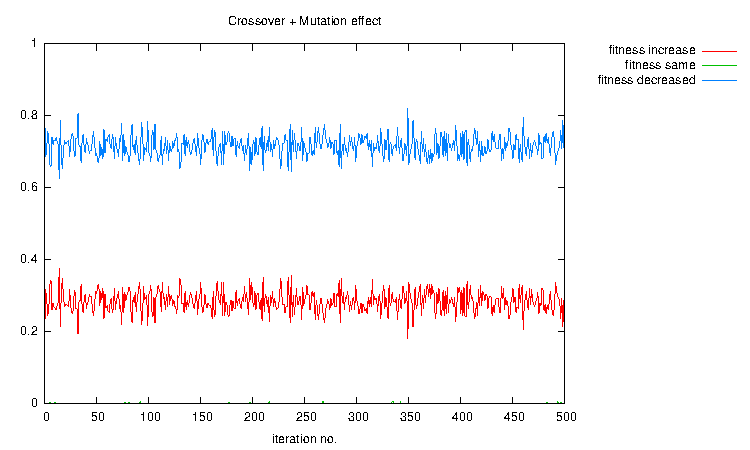
\includegraphics[width=0.8\textwidth]{results/4/1-cms.pdf}
\caption{Experiment 4: Total effect}
\label{pic-e4-cms}
\end{figure}


\subsection{Experiment 5}
Experiment 5 is similar to experiment 1, but with different CA rule.

\begin{verbatim}
Looking for rule: 1264947241 at radius: 2
Radius range: [1, 3]
Upscale probability: 0.1
Downscale probability: 0.1
Population count: 500
Mutation probability: 0.2
Max iteration count: 500
Space size: 79
Time frames: 80
Keep elite: true
Elite size: 4
\end{verbatim}

The overall results of this evolution is shown on picture \ref{pic-e5-results}. The measured effect of cross-over, mutation, and cross-over + mutation is shown on pictures: \ref{pic-e5-cs}, \ref{pic-e5-ms}, \ref{pic-e5-cms}.

\begin{figure}
\centering
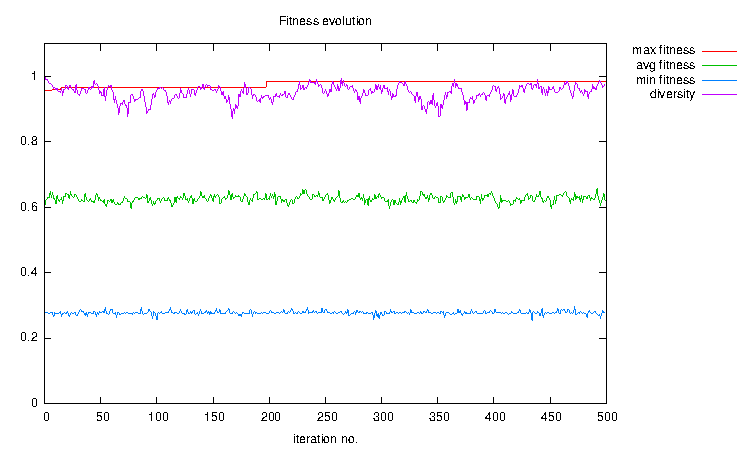
\includegraphics[width=0.8\textwidth]{results/5/1.pdf}
\caption{Experiment 5: Evolution results}
\label{pic-e5-results}
\end{figure}

\begin{figure}
\centering
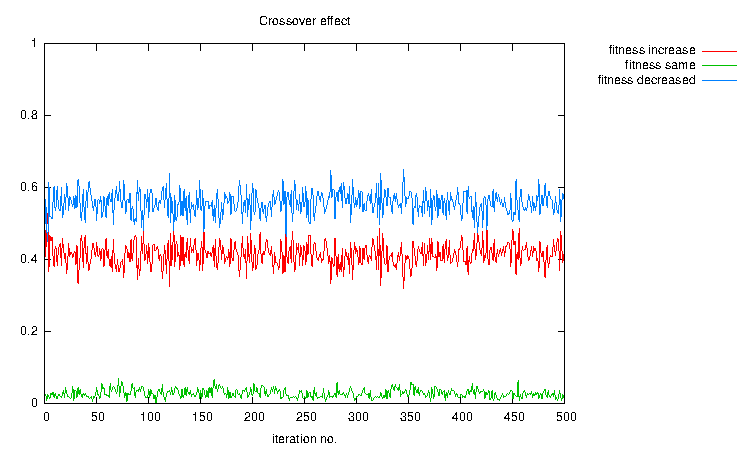
\includegraphics[width=0.8\textwidth]{results/5/1-cs.pdf}
\caption{Experiment 5: Crossover effect}
\label{pic-e5-cs}
\end{figure}

\begin{figure}
\centering
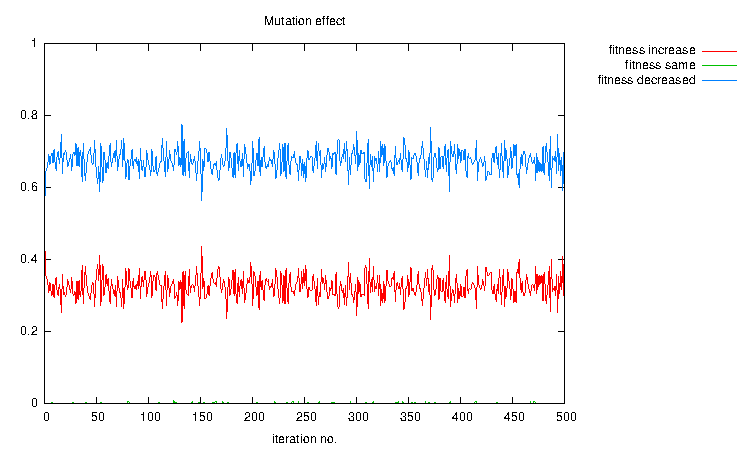
\includegraphics[width=0.8\textwidth]{results/5/1-ms.pdf}
\caption{Experiment 5: Mutation effect}
\label{pic-e5-ms}
\end{figure}

\begin{figure}
\centering
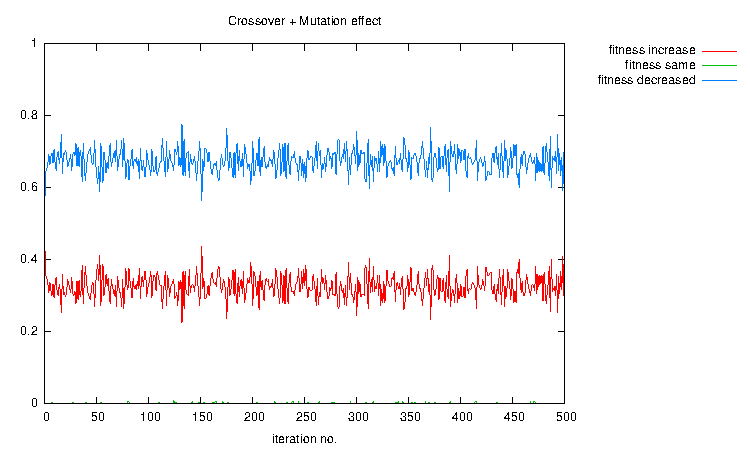
\includegraphics[width=0.8\textwidth]{results/5/1-cms.pdf}
\caption{Experiment 5: Total effect}
\label{pic-e5-cms}
\end{figure}

\section{Summary}
As seen on the plots negative or neutral effects dominate the evolution, meaning that bit-string CA rule representation with standard genetic operators is not an effective method for CA identification. Therefore other genetic operators and/or other rule representation schemes need to be used in future research.

\end{document}